\section{Ejecución del proyecto}
    \section{Diseño de Arquitectura de Negocio}
      \subsection{Punto de Vista Organizaciónal}
      El punto de vista de la organización se enfoca en el interior de la organización, un departamento, una red de empresas, es un punto de vista muy útil ya que permite identificar  competencias, autoridad y responsabilidades en una organización. \cite{ref9}
  \begin{table}[h]
	\centering
	\begin{tabular}{p{3.7cm}p{8cm}}
		\hline
        \textbf{Nombre} & \textbf{Organización} \\
		\hline
		\textbf{Stakeholders} & Organización, arquitectos de dominio y proceso, gerentes, empleados, accionistas.\\
		\textbf{Preocupaciones}v & Identificación de competencias, autoridad y responsabilidades.\\
		\textbf{Propósito} & Diseñar, decidir, informar. \\
		\textbf{Nivel de Abstracción} & Coherencia. \\
		\textbf{Capa} & Capa de negocio. \\
		\textbf{Aspectos} & Activo \\
	\end{tabular}
	\caption{Descripción Punto de Vista de la Organización \cite{ref9}}
	\label{tabla4}
  \end{table}
  \begin{figure}[h]
 	\centering
 	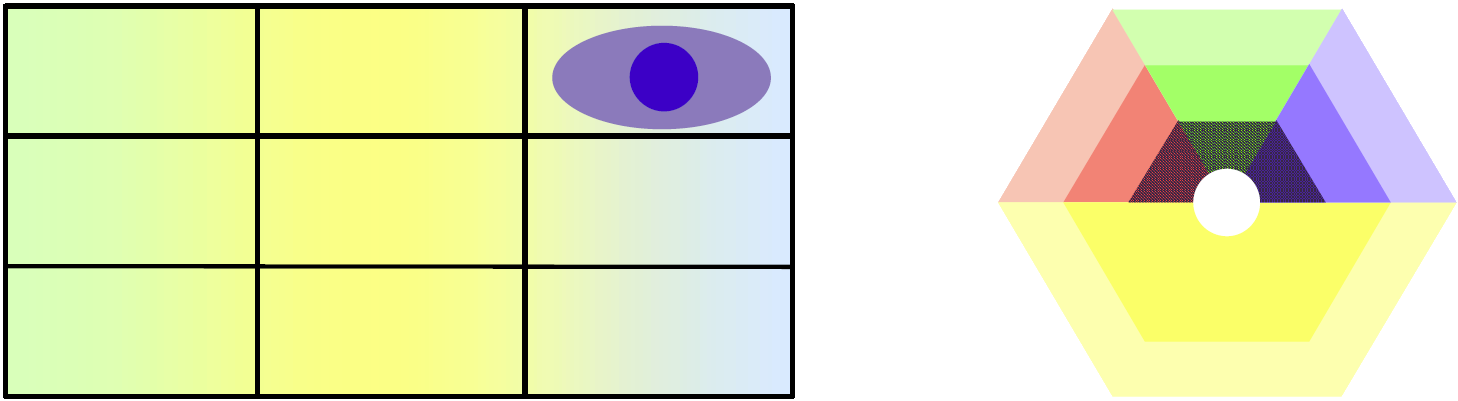
\includegraphics[scale=0.2]{Imagenes/Figuras/14.png}
 	\caption{Posición del punto de vista de organización conceptualmente y marco del punto de vista \cite{ref9}}
 	\label{figura14}
  \end{figure}
      \subsubsection{Metamodelo Punto de Vista Organizaciónal}
      La Figura \ref{metamodelo6} ilustra el punto de vista de producto el cual es la convergencia de los puntos de vista anteriores, es el esfuerzo por conocer la estructura, el esfuerzo por saber qué hace cada persona todo converge en el punto de vista que apunta al producto, el cual es un conjunto de servicios al cual se le adhiere un contrato y como elemento clave se le destaca un valor; el producto reposa sobre los procesos que son hechos por unos roles de negocio los cuales corresponden a unos actores. \cite{ref9}
  \begin{figure}[h]
	\centering
	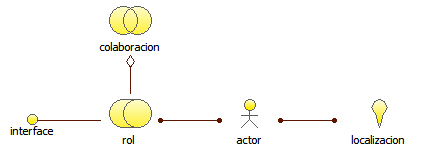
\includegraphics{Imagenes/Metamodelos/01.png}
	\caption{Metamodelo Punto de Vista de Producto \cite{ref9}}
	\label{metamodelo6}
  \end{figure}
      \subsubsection{Aplicación Punto de Vista Organizaciónal}
      \subsection{Punto de Vista de Cooperación}
      Este punto de vista se enfoca en los actores y sus relaciones con el entorno que los cobija, es un punto de vista donde los Stakeholders o interesados son la organización, los procesos y los arquitectos de dominio. La finalidad u objetivo de este punto de vista es la de diseñar, decidir e informar. \cite{ref9}

      \begin{table}[h]
      	\centering
      	\begin{tabular}{p{3.7cm}p{8cm}}
      		\hline
      		\textbf{Nombre} & \textbf{Cooperación} \\
      		\hline
      		\textbf{Stakeholders} & Organización, arquitectos de dominio y proceso \\
      		\textbf{Preocupaciones} & Relación de actores con el entorno \\
      		\textbf{Propósito} & Diseñar, decidir, informar \\
      		\textbf{Nivel} de Abstracción & Detalle \\
      		\textbf{Capa} & Capa de negocio \\
      		\textbf{Aspectos} & Estructura Activa, Comportamiento \\
      	\end{tabular}
      	\caption{Descripción Punto de Vista Cooperación de Actor \cite{ref9}}
      	\label{tabla5}
      \end{table}

      \begin{figure}[h]
      	\centering
      	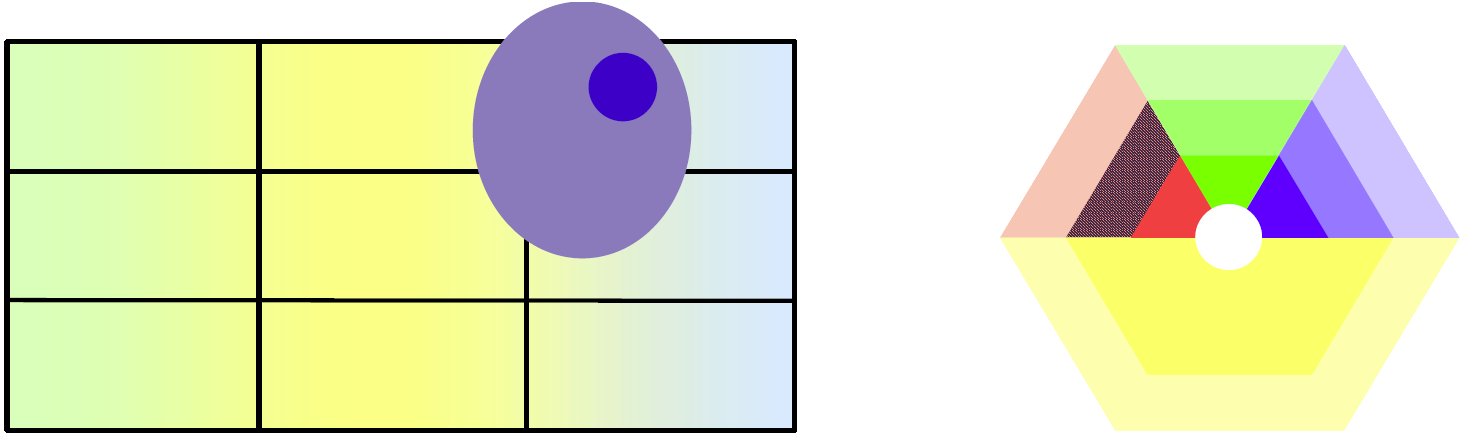
\includegraphics[scale=0.2]{Imagenes/Figuras/15.png}
      	\caption{Posición del punto de vista cooperación de actor conceptualmente y marco del punto de vista \cite{ref9}}
      	\label{figura15}
      \end{figure}
      \subsubsection{Metamodelo Punto de Vista Cooperación}
      En la Figura \ref{metamodelo2} se ilustra el metamodelo perteneciente al punto de vista de cooperación de actor el cual esta compuesto de los conceptos de actor, rol, interface, colaboración, servicio de negocio, servicio de aplicación, interface de comunicación de aplicación y componentes de aplicación.\\

      En este punto de vista a el actor se le asigna un rol, el rol se compone de interfaces, a la interface se le asigna servicios y estos servicios van a una capa de aplicación a través de una interface que está conformada por componentes de aplicación y es usada por componentes de aplicación. \\

      Otro uso importante del punto de vista de cooperación de actor es mostrar como un número de actores de negocio cooperantes y / o componentes de aplicación juntos realizan un proceso de negocio. Por lo tanto, en esta vista, tanto actores de negocio como roles y componentes de aplicación pueden aparecer. \cite{ref9}

      \begin{figure}[h]
      	\centering
      	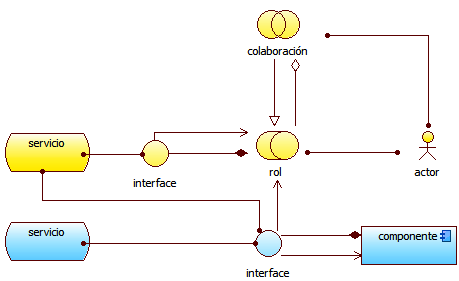
\includegraphics{Imagenes/Metamodelos/02.png}
      	\caption{Metamodelo Punto de Vista Cooperación de Actor \cite{ref9}}
      	\label{metamodelo2}
      \end{figure}
      \subsubsection{Aplicación Punto de Vista Cooperación}
      \section{Punto de Vista Función de Negocio}
      En este punto de vista se muestran las principales funciones de negocio de la organización y sus relaciones en términos de los flujos de información, valor, o productos entre ellas, los Stakeholders o interesados son los procesos y arquitectos de dominio, administradores operacionales, tiene especial cuidado en la estructura de los procesos de negocio, su coherencia, integridad y las responsabilidades. \cite{ref9}

      \begin{table}[h]
      	\centering
      	\begin{tabular}{p{3.7cm}p{8cm}}
      		\hline
      		\textbf{Nombre} & \textbf{Función de Negocio}\\
      		\hline
      		\textbf{Stakeholders} & Organización, arquitectos de dominio y proceso \\
      		\textbf{Preocupaciones} & Identificación de competencias, identificación de actividades principales, reducción de la complejidad \\
      		\textbf{Propósito} & Diseñar \\
      		\textbf{Nivel de Abstracción} & Coherencia \\
      		\textbf{Capa} & Capa de negocio \\
      		\textbf{Aspectos} & Comportamiento (Activo) \\
      	\end{tabular}
      	\caption{Descripción Punto de Vista Función de Negocio}
      	\label{Tab:tabla6}
      \end{table}

      \begin{figure}[h]
      	\centering
      	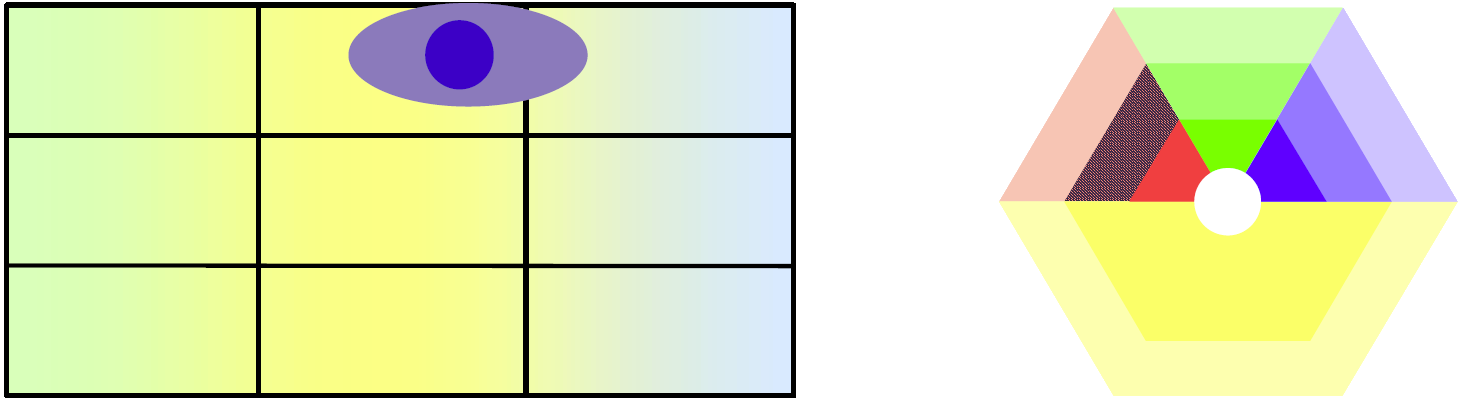
\includegraphics[scale=0.2]{Imagenes/Figuras/16.png}
      	\caption{Posición del punto de vista función de negocio conceptualmente y marco del punto de vista \cite{ref9}}
      	\label{figura16}
      \end{figure}

      \subsection{Metamodelo}
      La Figura \ref{metamodelo3} muestra los conceptos de actor, rol y función; aquí se asignan tareas o funciones a estos actores, en el modelo se extrae lo que interesa, lo que se quiere capturar o tener en la mente. En este metamodelo aparecen dos tipos de relaciones el flujo y los disparos. \cite{ref9}

      \begin{figure}[h]
      	\centering
      	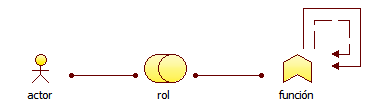
\includegraphics{Imagenes/Metamodelos/03.png}
      	\caption{Metamodelo}
      	\label{metamodelo3}
      \end{figure}

      \section{Punto de Vista Proceso}
      El punto de vista de proceso de negocio es el encargado de mostrar una estructura de alto nivel y composición de uno o más procesos de negocio. Tiene una complejidad importante, se incorporan elementos de comportamiento se incluye el proceso y/o función de negocio como elemento central, el proceso y/o función de negocio se ve afectado por las mismas relaciones con los demás conceptos, este punto de vista llama la atención en que nos induce a las entrañas de las organizaciones porque se ve lo que ellas hacen. \cite{ref9}

      \begin{table}[h]
      	\centering
      	\begin{tabular}{p{3.7cm}p{8cm}}
      		\hline
      		\textbf{Nombre} & \textbf{Proceso} \\
      		\hline
      		\textbf{Stakeholders} & Arquitectura de dominio y proceso, Gerentes de operación \\
      		\textbf{Preocupaciones} & Estructurar los procesos del negocio, consistencia, integridad y responsabilidades \\
      		\textbf{Propósito} & Diseñar \\
      		\textbf{Nivel de Abstracción} & Detalle \\
      		\textbf{Capa} & Capa de negocio \\
      		\textbf{Aspectos} & Comportamiento (Activo), (Pasivo) \\
      	\end{tabular}
      	\caption{Descripción punto de vista proceso de negocio \cite{ref9}}
      	\label{Tab:tabla7}
      \end{table}

      \begin{figure}[h]
      	\centering
      	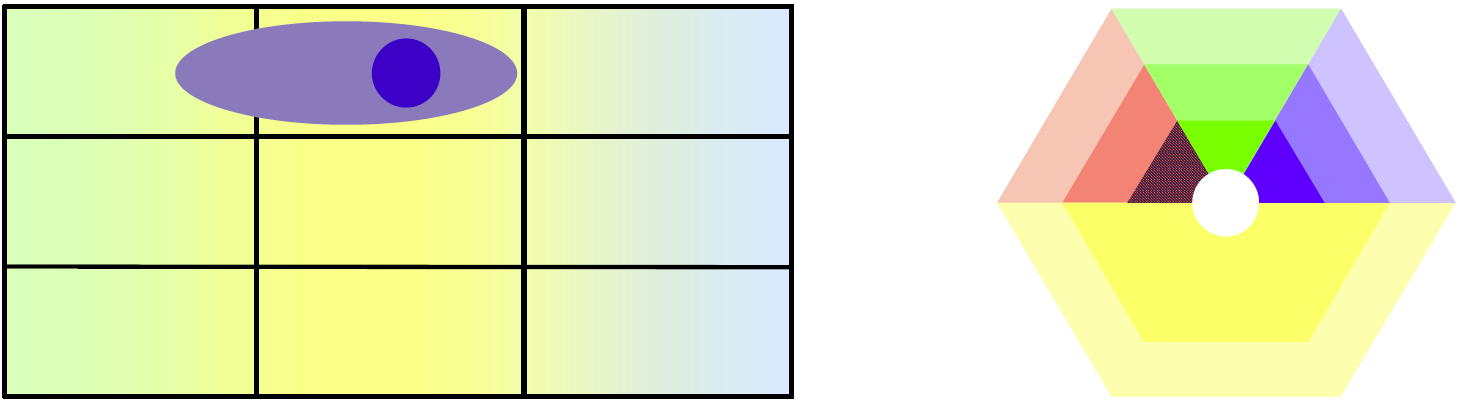
\includegraphics[scale=0.2]{Imagenes/Figuras/17}
      	\caption{Posición del punto de vista proceso de negocio conceptualmente y marco del punto de vista \cite{ref9}}
      	\label{figura17}
      \end{figure}

      \subsection{Metamodelo}
      La Figura \ref{metamodelo4} se aprecia que el proceso de negocio tiene que ver con un rol o conjunto de roles, el proceso de negocio es disparado por un evento y el proceso de negocio genera un evento o un proceso de eventos, los procesos no son máquinas infinitas todo proceso es
      iniciado por uno o un conjunto de eventos.

      Los procesos generan objetos de negocio que es la representación del trabajo en la organización,  el servicio de negocio es lo que el proceso de negocio lleva a cabo estableciéndose entre los dos una relación de realización, el servicio es el core de negocio lo que el cliente mira, el proceso de negocio es lo que implementa realiza, materializa el servicio y el proceso de negocio funciona porque existen unos roles que se encargan de realizar el proceso. \cite{ref9}

      \begin{figure}[h]
      	\centering
      	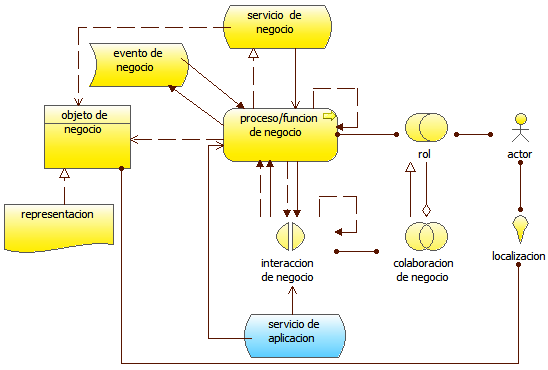
\includegraphics{Imagenes/Metamodelos/04.png}
      	\caption{Metamodelo}
      	\label{metamodelo4}
      \end{figure}

      \section{Punto de Vista Cooperación}
      El punto de vista de cooperación de proceso de negocio es usado para mostrar las relaciones
      de uno o mas procesos de negocio con los demás procesos de negocio y / o con su ambiente. Puede ser usado tanto para crear un diseño de alto nivel de procesos de negocio dentro de su contexto como para proveer un responsable administrador operacional para uno o mas de tales procesos con mando en sus dependencias. \cite{ref9}

      \begin{table}[h]
      	\centering
      	\begin{tabular}{p{3.7cm}p{8cm}}
      		\hline
      		\textbf{Nombre} & \textbf{Cooperación} \\
      		\hline
      		\textbf{Stakeholders} & Arquitectos de domino, Gerentes de Operaciones \\
      		\textbf{Preocupaciones} & Dependencias de los procesos de negocio, Responsabilidades \\
      		\textbf{Propósito} & Diseñar, decidir \\
      		\textbf{Nivel} de Abstracción \\
      		\textbf{Capa} & Capa de Negocio) \\
      		\textbf{Aspectos} & Comportamiento, (activo), (pasivo) \\
      	\end{tabular}
      	\caption{Descripción punto de vista de cooperación de proceso \cite{ref9}}
      	\label{tabla8}
      \end{table}

      \begin{figure}[h]
      	\centering
      	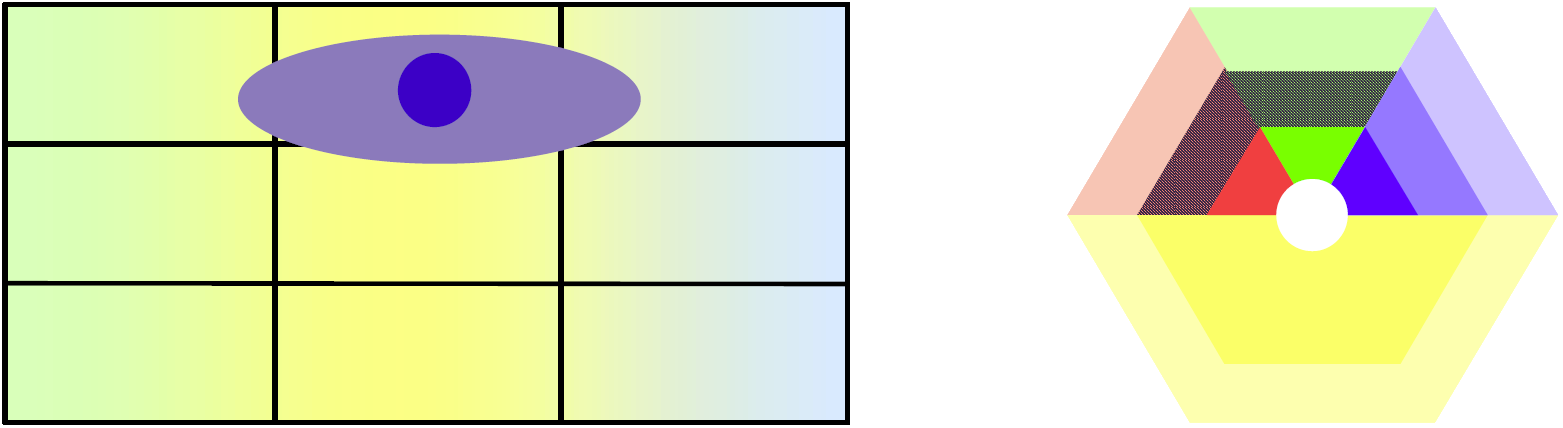
\includegraphics[scale=0.2]{Imagenes/Figuras/18.png}
      	\caption{Posición del punto de vista de cooperación de proceso conceptualmente y marco del punto de vista \cite{ref9}}
      	\label{figura18}
      \end{figure}

      \subsection{Metamodelo}
      En la Figura \ref{metamodelo5} se ilustra el metamodelo perteneciente al punto de vista de cooperación de proceso el cual esta compuesto de los conceptos de los procesos del negocio y sus responsabilidades. En este punto de vista a al proceso se le asigna un rol, el rol se compone de interfaces, a la interface se le asigna interacciones y estas interacciones van a una capa de aplicación a través de una interface. \cite{ref9}

      \begin{figure}[h]
      	\centering
      	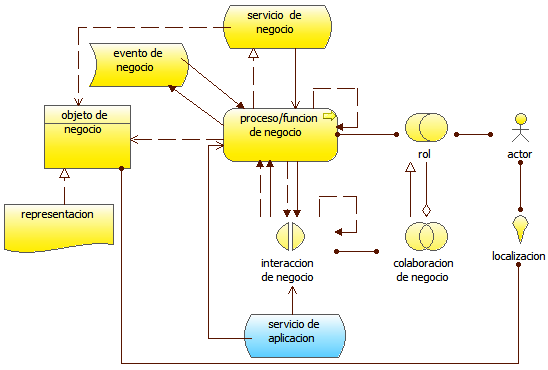
\includegraphics{Imagenes/Metamodelos/05.png}
      	\caption{Metamodelo}
      	\label{metamodelo5}
      \end{figure}

      \section{Punto de Vista de Producto}
      Este punto de vista se describe como eje central el valor que uno o más productos ofrecen a la clientes u otras partes externas involucradas con la organización, muestra además la composición de uno o más productos en términos de cómo están compuestos, la asociación, el contrato y otros acuerdos. El punto de vista del producto se suele utilizar en el desarrollo de productos para diseñar un producto componiendo servicios existentes o mediante la identificación de nuevos servicios que se tienen que crear para este producto, dado el valor que un cliente espera de ella. \cite{ref9}

      \begin{table}[h]
      	\centering
      	\begin{tabular}{p{3.7cm}p{8cm}}
      		\hline
      		\textbf{Nombre} & \textbf{Vista de Producto} \\
      		\hline
      		\textbf{Stakeholders} & Diseñadores de producto, gerentes de producto, Arquitectos de proceso y de dominio \\
      		\textbf{Preocupaciones} & Desarrollo del producto y el valor que este ofrece a la organización \\
      		\textbf{Propósito} & Diseñar, decidir \\
      		\textbf{Nivel de Abstracción} & Coherencia \\
      		\textbf{Capa} & Capa de Negocio \\
      		\textbf{Aspectos} & Comportamiento, información, (activo) \\
      	\end{tabular}
      	\caption{Descripción Punto de Vista de Producto}
      	\label{tabla9}
      \end{table}

      \begin{figure}[h]
      	\centering
      	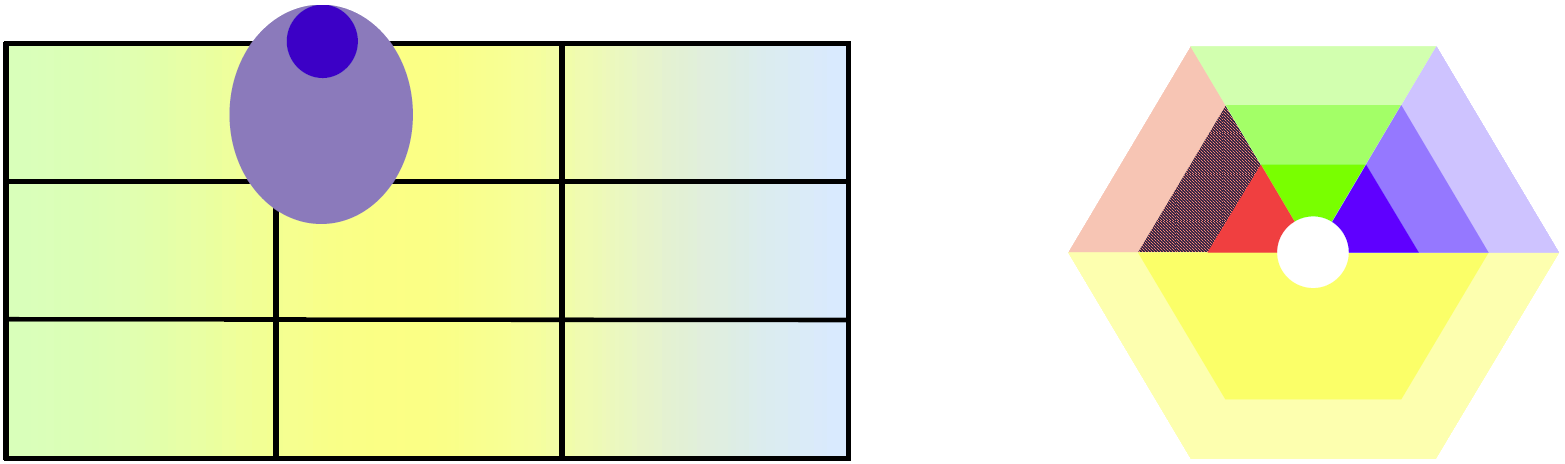
\includegraphics[scale=0.2]{Imagenes/Figuras/19.png}
      	\caption{Posición del Punto de Vista de Producto}
      	\label{figura19}
      \end{figure}

      \subsection{Metamodelo}
      La Figura \ref{metamodelo6} ilustra el punto de vista de producto el cual es la convergencia de los puntos de vista anteriores, es el esfuerzo por conocer la estructura, el esfuerzo por saber qué hace cada persona todo converge en el punto de vista que apunta al producto, el cual es un conjunto de servicios al cual se le adhiere un contrato y como elemento clave se le destaca un valor; el producto reposa sobre los procesos que son hechos por unos roles de negocio los cuales corresponden a unos actores. \cite{ref9}

      \begin{figure}[h]
      	\centering
      	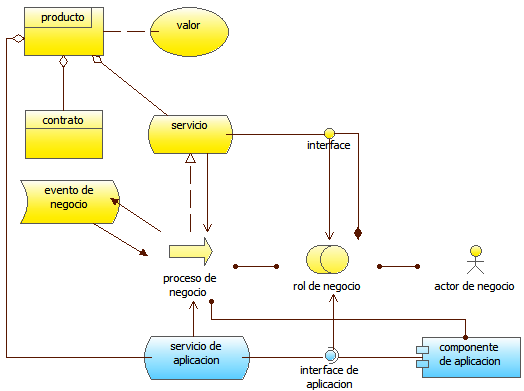
\includegraphics{Imagenes/Metamodelos/06.png}
      	\caption{Metamodelo}
      	\label{metamodelo6}
      \end{figure}
     \section{Diseño de Arquitectura de Aplicación}
      \subsection{Punto de Vista Comportamiento de Aplicación}
      \subsubsection{Metamodelo de Punto de Vista de Comportamiento de Aplicación}
      \subsubsection{Aplicación Punto de Vista de Comportamiento de Aplicación}
      \subsection{Punto de Vista Cooperación de Aplicación}
      \subsubsection{Metamodelo de Punto de Vista de Cooperación de Aplicación}
      \subsubsection{Aplicación Punto de Vista de Cooperación de Aplicación}
      \subsection{Punto de Vista Estructura de Aplicación}
      \subsubsection{Metamodelo de Punto de Vista de Estructura de Aplicación}
      \subsubsection{Aplicación Punto de Vista de Cooperación de Aplicación}
      \subsection{Punto de Vista Uso de Aplicación}
      \subsubsection{Metamodelo de Punto de Vista de Uso de Aplicación}
      \subsubsection{Aplicación Punto de Vista de Cooperación de Aplicación}
     \section{Diseño de Arquitectura de Infraestructura y Datos ˜}
      \subsection{Punto de Vista de Infraestructura}
      \subsubsection{Metamodelo de Punto de Vista de Infraestructura}
      \subsubsection{Aplicación Punto de Vista de Infraestructura}
      \subsection{Punto de Vista de Uso de Infraestructura}
      \subsubsection{Metamodelo de Punto de Vista de Uso de Infraestructura}
      \subsubsection{Aplicación Punto de Vista de Uso de Infraestructura}
      \subsection{Punto de Vista Organización e implementación}
      \subsubsection{Metamodelo de Punto de Vista de Organización e implementación}
      \subsubsection{Aplicación Punto de Vista de Organización e implementación}
      \subsection{Punto de Vista Estructura de Información}
      \subsubsection{Metamodelo de Punto de Vista de Estructura de Información}
      \subsubsection{Aplicación Punto de Vista de Estructura de Información}
      \subsection{Punto de Vista de Realización del Servicio}
      \subsubsection{Metamodelo de Punto de Vista de Realización del Servicio}
      \subsubsection{Aplicación Punto de Vista de Realización del Servicio}
      \subsection{Punto de Vista de Capas}
      \subsubsection{Metamodelo de Punto de Vista de Capas}
      \subsubsection{Aplicación Punto de Vista de Capas}
     \section{Diseño de Arquitectura Motivacional}
      \subsection{Punto de Vista de Stakeholder}
      \subsubsection{Metamodelo de Punto de Vista de Stakeholder}
      \subsubsection{Aplicación de Punto de Vista de Stakeholder}
      \subsection{Punto de Vista de Realización de Objetivos}
      \subsubsection{Metamodelo de Punto de Vista de Realización de Objetivos}
      \subsubsection{Aplicación de Punto de Vista de Realización de Objetivos}
      \subsection{Punto de Vista de Contribución}
      \subsubsection{Metamodelo de Punto de Vista de Contribución}
      \subsubsection{Aplicación Punto de Vista de Contribución}
      \subsection{Punto de Vista de Principios}
      \subsubsection{Metamodelo de Punto de Vista de Principios}
      \subsubsection{Aplicación Punto de Vista de Principios}
      \subsection{Punto de Vista de Realización de Requerimientos}
      \subsubsection{Metamodelo de Punto de Vista de Realización de Requerimientos}
      \subsubsection{Aplicación Punto de Vista de Realización de Requerimientos}
      \subsection{Punto de Vista de Motivación}
      \subsubsection{Metamodelo de Punto de Vista de Motivación}
      \subsubsection{Aplicación Punto de Vista de Motivación}
     \section{Diseño de Arquitectura de Proyecto}
      \subsection{Punto de Vista de Proyecto}
      \subsubsection{Metamodelo de Punto de Vista de Proyecto}
      \subsubsection{Aplicación de Punto de Vista de Proyecto}
      \section{Diseño de Arquitectura de Migración}
      \subsection{Punto de Vista de Migración}
      \subsubsection{Metamodelo de Punto de Vista de Migración}
      \subsubsection{Aplicación de Punto de Vista de Migración}
      \subsection{Punto de Vista de Migración e Implementación}
      \subsubsection{Metamodelo de Punto de Vista de Migración e Implementación}
      \subsubsection{Aplicación de Punto de Vista de Migración e Implementación}
